\chapter[Projeto de Processos]{Projeto de Processos}
\label{chap:processos}

	\section[Definição]{Definição}
	\label{sec:processos_definicao}
	
		Não existe uma definição precisa para “projeto” em que seja reconhecida universalmente, mas segundo \cite{sir}: 

		\begin{quotation}
			“Em minha definição, projeto é o processo conceitual através do qual algumas exigências funcionais de pessoas, individualmente ou em massa, são satisfeitas através do uso de um produto ou de um sistema que representa a tradução física do conceito. Como exemplos de produtos individuais que satisfazem a uma necessidade pública ou de mercado temos o automóvel, a televisão e o rádio, a geladeira e a lavadora de pratos, sapatos e meias, e fraldas para bebês, mas também a pintura, a escultura, a música e as muitas outras manifestações de expressão do artista etc.; e como sistemas há o telefone e a ferrovia, a rodovia e o supermercado, a orquestra, o fornecimento de utilidades (gás, água e eletricidade) e assim por diante.”
		\end{quotation}

		A partir dessa definição é possível ser extraído alguns pontos importante:

		\begin{itemize}
			\item{O objetivo da atividade de projeto é satisfazer às necessidades dos consumidores;}
			\item{A atividade de projeto aplica-se tanto a produtos ou serviços, como em um sistema ou processo;}
			\item{A atividade de projeto é em si mesma um processo de transformação;}
			\item{O projeto começa com um conceito e termina na tradução desse conceito em uma especificação de algo que pode ser produzido.}
		\end{itemize}

		Mas, a principal questão a ser identificada é: \emph{qual a finalidade de projeto de processos?} Simples, é planejar os sistemas a serem utilizados para execução dos produtos/serviços desejados. O Projeto de Produtos/Serviços e o Projeto dos Processos que os produzem estão intimamente inter-relacionados, como ilustra a imagem a seguir:

		\begin{figure}[h]
			\centering
			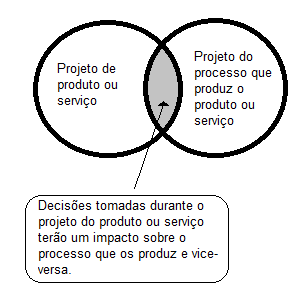
\includegraphics[scale=0.7]{processo1}
			\caption[Inter-relacionados entre projeto de produtos e projeto de processos]{Inter-relacionados entre projeto de produtos e projeto de processos.}
			\label{fig:processo1}
		\end{figure}

		Duas características intrínsecas entre são o \textbf{volume-variedade}. Esse binômio é pioneiro no que desrespeito as abordagens gerais para gerenciamentos de processos. Logo, a partir disso, define-se o tipo de processo no qual caracterizam a forma de produção do produto ou serviço. Nas próximas seções, serão abordadas esses tipos de processos.

		\section[Processos em Manufatura]{Processos em Manufatura}
		\label{sec:processos_manufatura}
			
			A ilustração a seguir apresenta a divisão segundo \cite{slack} para o processo manufaturado.

			\begin{figure}[h]
				\centering
				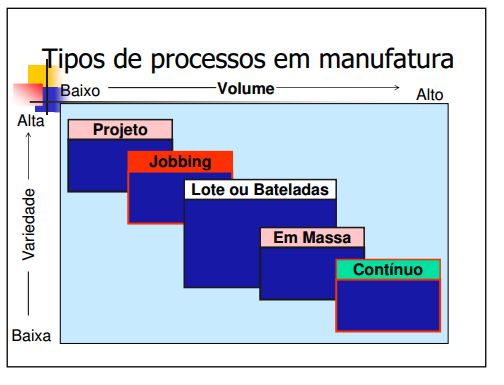
\includegraphics[scale=0.9]{processo2}
				\caption[Tipos de processos em Manufatura]{Tipos de processos em Manufatura.}
				\label{fig:processo2}
			\end{figure}

			Na manufatura, isto é, na produção de produtos são definidos os seguintes processo:

			\subsection[Processos de Projeto]{Processos de Projeto}
			\label{sec:processos_manufatura_projeto}

				Lidam com produtos discretos, no qual são extremamente personalizados. Normalmente o tempo para produzir ou construir é longo possuindo um baixo volume é uma altíssima variedade.
				
				\emph{Ex.:} Grandes projetos – navio, edifício, túnel, viaduto, etc.

			\subsection[Processos de Jobbing]{Processos de \emph{Jobbing}}
			\label{sec:processos_manufatura_jobbing}

				A produção dos produtos envolve o compartilhamento dos recursos de operação com o produto em produção. Normalmente é produzido em baixo volume e também com um alta índice de variedade.
				
				\emph{Ex.:} Técnicos especializados, restauradores de móveis, alfaiates (por encomenda), gráfica (ingressos para determinados eventos), etc

			\subsection[Processos em Lotes ou Bateladas]{Processos em Lotes ou Bateladas}
			\label{sec:processos_manufatura_lotes}

				Para cada vez que um processo em lote produz um produto, é produzido mais do que um produto. Normalmente produz mais de um produto com um grau médio de variedade.
				
				\emph{Ex.:} Alimentos congelados especiais, fabricação de peças componentes, etc.

			\subsection[Processos de Produção em Massa]{Processos de Produção em Massa}
			\label{sec:processos_manufatura_massa}

				São os que produzem bens em alto volume e variedade relativamente estreita. Normalmente lidam com atividades repetitivas e produtos padronizados, além disso possuem altos volumes e baixa variedade.
				
				\emph{Ex.:} Montadoras de automóveis, fabricação de bens duráveis, confecção de pizza congelada, produção de CD’s, etc.

			\subsection[Processos de Produção em Massa]{Processos de Produção em Massa}
			\label{sec:processos_manufatura_massa}

				Situam-se um passo além dos processos de produção em massa, pelo fato de operarem em volumes ainda maiores e em geral terem variedade ainda mais baixa. Normalmente operam por períodos de tempo muito mais longos de modo contínuo (24 horas/dia).
				
				\emph{Ex.:} Refinarias de petróleo, siderúrgicas, fábrica de papéis, hidroelétricas, etc.

		\section[Processos de Operações de Serviços]{Processos de Operações de Serviços}
		\label{sec:processos_servico}

			A ilustração a seguir apresenta a divisão segundo \cite{slack} para o processo de prestação de serviço.

			\newpage
			\begin{figure}[h]
				\centering
				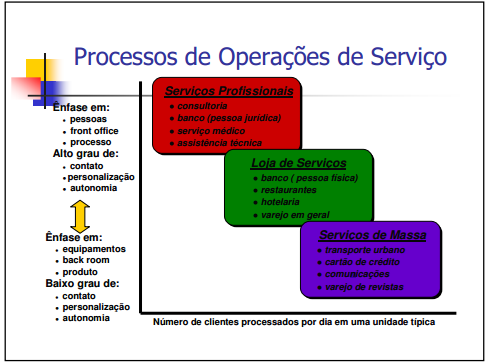
\includegraphics[scale=0.9]{processo3}
				\caption[Tipos de processos em Serviços]{Tipos de processos em Serviços.}
				\label{fig:processo3}
			\end{figure}

			Agora, para a prestação de serviço são definidos os seguintes processo:

			\subsection[Serviços Profissionais]{Serviços Profissionais}
			\label{sec:processos_servico_profissionais}

				Baseados em pessoas e ênfase no processo, isto é, como o serviço é prestado. Cada projeto é diferente e alta customização implicando em um atendimento personalizado.
				
				\emph{Ex.:} Consultores de gestão, advogados, arquitetos, cirurgiões, auditores, etc.

			\subsection[Loja de Serviços]{Loja de Serviços}
			\label{sec:processos_servico_loja}

				Baseado no equilíbrio entre produtos e processos. Normalmente possui níveis de contato com o cliente, são customização, além de terem um volume de clientes e liberdade de decisão do pessoal que atende/presta o serviço.
			
				\emph{Ex.:} Bancos, lojas, restaurantes, operadoras de turismo e lazer, escolas, hotéis, etc.

			\subsection[Serviços de Massa]{Serviços de Massa}
			\label{sec:processos_servico_massa}

				Baseado em equipamentos e ênfase no produto que é fornecido. Normalmente compreendem muitas transações de clientes que envolvem tempo de contato limitado e pouca customização.
				
				\emph{Ex.:} Supermercados, aeroportos, livrarias, emissoras de televisão, polícia, serviço público, etc. 

	\section[Aplicações]{Aplicações - \begin{figure}[h]
\includegraphics{bobs}\end{figure}}
	\label{sec:processos_aplicacoes}

		De acordo com o livro de \cite{lamonica}, no qual verifica-se a biografia da rede \textbf{Bob’s}, Robert Falkenburg, criador da rede, carinhosamente chamado de Bob, possuía em seu projeto de processo se baseava em 3 diretrizes: \textbf{serviço rápido}, sempre a \textbf{melhor qualidade} no \textbf{produto} e na \textbf{limpeza}. Nos anos 50, ele sozinho cuidou de sua loja com as 3 diretrizes citadas acima e um trunfo a mais que era ouvir o seu cliente. O que ajudou muito no desenvolvimento da companhia foi a participação de Robert em todo o projeto de rede da sua loja. Ele ia em busca da qualidade, não querendo ter dependência de nada nem ninguém para que seu produto fosse o melhor do mercado. Falkenburg foi o pioneiro do \emph{fast food} no Brasil.

		Nos anos 60, Robert transfere o poder acionário da sua marca para a Libby do Brasil que posteriormente começa a ser representada pela BFFC. Ao longo dos mais de 60 anos de existência, mudaram-se os processos da companhia. Hoje a BFFC tem como carro-chefe o projeto "5P", que significa \emph{Product, Price, Place, Promotion e People} (Produto, preço, lugar, promoção e pessoas).

		Atualmente os restaurantes de \emph{fast food} da rede da \textbf{Bob’s} se encaixam nas lojas de serviço definida segundo \cite{slack}:

		\begin{quotation}
			“Lojas de serviços são caracterizadas por níveis de contato com o cliente, customização, volumes de clientes e liberdade de decisão do pessoal, que as posiciona entre os extremos do serviço profissional e de massa. O serviço é proporcionado por meio de combinações de atividades dos escritórios da linha de frente e da retaguarda, pessoas e equipamentos e ênfase no produto/processo.” 
		\end{quotation}

		No entanto, a empresa não oferece apenas serviços. Quando observasse a essência de sua natureza, nota-se uma produção em massa de sanduiches. De fato, os restaurantes de \emph{fast food} são caracterizados pela produção em grande escala de sanduiches e secundariamente \emph{milk shakes}, pratos prontos entre outros. Ambas características são importantes, pois tem impactos no marketing da empresa como por exemplo no projeto 5P do \textbf{Bob’s}.

		O Projeto 5P foi criado depois de uma pesquisa grande e qualitativa com clientes que queriam a melhoria dos processos e produtos no \textbf{Bob’s}. Tem dado certo. Nos últimos anos o \textbf{Bob’s} alcançou a marca de mais de 1 milhão de litros de \emph{milk shakes} vendidos por mês pela franquia em todo o mundo.




	
